\documentclass[tikz]{standalone}

\usepackage[T1]{fontenc}
\usepackage[english]{babel}

\usepackage{bm, amsmath, mleftright}
\usepackage{graphicx}

\NewDocumentCommand{\evalat}{sO{\big}mm}{%
    \IfBooleanTF{#1}
    {\mleft. #3 \mright|_{#4}}
    {#3#2|_{#4}}%
}


\usepackage{tikz}
\usetikzlibrary{trees, calc}

\begin{document}
    \tikzstyle{level 1}=[level distance=3cm, sibling distance=3cm]
    \tikzstyle{level 2}=[level distance=4cm, sibling distance=2cm]
    
    \tikzstyle{signal}=[rounded corners, draw, align=center]
    \tikzstyle{unamed}=[draw, circle]

    \begin{tikzpicture}[grow=south]
        \node (x) {
\includegraphics[width=3cm]{images/scatnet/x}}
            child[magenta, visible on=<4->]{
                node[unamed] (x1_1) {}
                child[magenta, visible on=<8->]{
                    node[unamed] (x1_1_1) {}
                }
                child[magenta, visible on=<8->]{
                    node (x1_1_2) {\dots}
                }
                child[magenta, visible on=<8->]{
                    node[unamed] (x1_1_3) {}
                }
            }
            child[magenta, visible on=<4->]{
                node (x1_2) {\dots}
            }
            child[magenta, visible on=<4->]{
                node[unamed] (x1_3) {}
                child[magenta, visible on=<8->]{
                    node[unamed] (x1_3_1) {}
                }
                child[magenta, visible on=<8->]{
                    node (x1_3_2) {\dots}
                }
                child[magenta, visible on=<8->]{
                    node[unamed] (x1_3_3) {} edge from parent node[midway, right, align=center, draw=none, visible on=<8>] {
                        $\left\lvert \bullet \ostar_{SE(2)} \psi_{i_2, \xi_2, \theta_2}\right\rvert$\\
                        \footnotesize $i_2 = 1, 2, \dots, I$\\
                        $\xi_2= 1, 2, \dots, \lfloor\log_2(L)\rfloor$\\
                        $\theta_2 = 1, 2, \dots, L$
                    }
                } edge from parent node[midway, right, align=center, draw=none, visible on=<4>] {
                    $\left\lvert \bullet \star \psi_{i_1, \theta_1}\right\rvert$\\
                    \footnotesize $i_1 = 1, 2, \dots, I$\\
                    $\theta_1 = 1, 2, \dots, L$
                }
            };

            \path (x.south) + (0, -2) node[signal, blue, anchor=north, visible on=<2>] (s0) {\small $S_0[x]$};
            \path[draw, blue, ->, visible on=<2>] (x.south) -- (s0) node[midway, left] {$\phi_I$};
            \path[draw, blue, ->, visible on=<3>] (x.south) -- ($(x.south) + (0, -1)$) node[anchor=north] {
\includegraphics[width=2cm]{images/scatnet/s0}};
            \path[draw, blue, ->, visible on=<4->] (x.200) -- ($(x.200) + (-2, -1)$) node[signal, anchor=north east] (s0) {\small $S_0[x]$};

            \path (x1_1.south west) + (-1, -.5) node[signal, blue, anchor=north east, visible on=<5>] (s1_1) {\small $\evalat[\Bigg]{S_1[x]}{i_1, \theta_1}$};
            \path[draw, blue, ->, visible on=<5>] (x1_1.200) -- (s1_1) node[midway, left] {$\phi_I$};
            \path[draw, blue, ->, visible on=<5>] (x1_3.200) -- ($(x1_3.south west) + (-1, -.5)$) node[anchor=north east] (s1_3) {};
            \path[draw, blue, ->, visible on=<6>] (x1_2.south) -- ($(x1_2.south) + (0, -1)$) node[anchor=north] (s1) {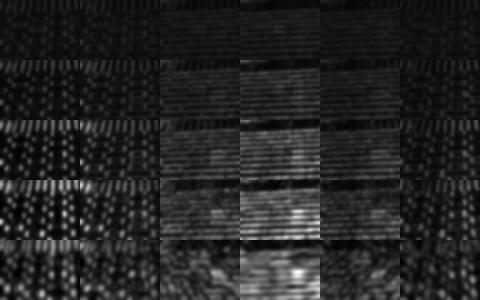
\includegraphics[width=6cm]{images/scatnet/s1}};
            \path[draw, blue, ->, visible on=<7->] (x1_1.200) -- ($(x1_1.south west) + (-1, -.5)$) node[signal, anchor=north east] {\small $\evalat[\Bigg]{S_1[x]}{i_1, \theta_1}$};
            \path[draw, blue, ->, visible on=<7->] (x1_3.200) -- ($(x1_3.south west) + (-1, -.5)$) node[anchor=north east] (s1_3) {};

            \path (x1_1_1.south west) + (-1, -.5) node[signal, anchor=north east, blue, visible on=<9>] (s1_1_1) {\small $\evalat[\Bigg]{S_2[x]}{i_1, \theta_1, i_2,\xi_2, \theta_2}$};
            \path[draw, blue, ->, , visible on=<9>] (x1_1_1.200) -- (s1_1_1) node[midway, left] {$\phi_I$};
            \path[draw, blue, ->, , visible on=<9>] (x1_1_3.200) -- ($(x1_1_3.south west) + (-1, -.5)$) node[anchor=north east] (s1_1_3) {};
            \path[draw, blue, ->, , visible on=<9>] (x1_3_1.200) -- ($(x1_3_1.south west) + (-1, -.5)$) node[anchor=north east] (s1_3_1) {};
            \path[draw, blue, ->, , visible on=<9>] (x1_3_3.200) -- ($(x1_3_3.south west) + (-1, -.5)$) node[anchor=north east] (s1_3_3) {};
            \path[visible on=<10>] ($(x1_1_3.south)!.5!(x1_3_1.south)$) + (0, -.5) node[anchor=south] (s2) {
\includegraphics[width=12cm]{images/scatnet/s2}};

            \path[draw, blue, ->, visible on=<11->] (x1_1_1.200) -- ($(x1_1_1.south west) + (-1, -.5)$) node[signal, anchor=north east] (s1_1_1) {\small $\evalat[\Bigg]{S_2[x]}{i_1, \theta_1, i_2, \xi_2, \theta_2}$};
            \path[draw, blue, ->, , visible on=<11->] (x1_3_1.200) -- ($(x1_3_1.south west) + (-1, -.5)$) node[anchor=north east] (s1_3_1) {};
            \path[draw, blue, ->, , visible on=<11->] (x1_3_3.200) -- ($(x1_3_3.south west) + (-1, -.5)$) node[anchor=north east] (s1_3_3) {};
        \end{tikzpicture}
\end{document}
